\documentclass[12pt,letterpaper]{article}
\usepackage[latin1]{inputenc}
\usepackage{amsmath}
\usepackage{amsfonts}
\usepackage{amssymb}

% the above packages are the "base"

\usepackage{graphicx}

\usepackage{hyperref} % enable links within pdf
\hypersetup{colorlinks = true, linkcolor = black, urlcolor = blue}

\usepackage{bm}
\usepackage{xcolor}

\usepackage{float} % for hard H placement of figures

\usepackage{fancyvrb}

\usepackage{listings} % to typeset in R format
\xdefinecolor{gray}{rgb}{0.4,0.4,0.4}
\xdefinecolor{blue}{RGB}{58,95,205}% R's royalblue3; #3A5FCD
\lstset{% setup listings
	language=R,% set programming language
	basicstyle=\ttfamily\small,% basic font style
	keywordstyle=\color{blue},% keyword style
	commentstyle=\color{gray},% comment style
	numbers=left,% display line numbers on the left side
	numberstyle=\scriptsize,% use small line numbers
	numbersep=10pt,% space between line numbers and code
	tabsize=3,% sizes of tabs
	showstringspaces=false,% do not replace spaces in strings by a certain character
	captionpos=b,% positioning of the caption below
	breaklines=true,% automatic line breaking
	escapeinside={(*}{*)},% escaping to LaTeX
	fancyvrb=true,% verbatim code is typset by listings
	extendedchars=false,% prohibit extended chars (chars of codes 128--255)
%	literate={"}{{\texttt{"}}}1{<-}{{$\bm\leftarrow$}}1{<<-}{{$\bm\twoheadleftarrow$}}1
%	{~}{{$\bm\sim$}}1{<=}{{$\bm\le$}}1{>=}{{$\bm\ge$}}1{!=}{{$\bm\neq$}}1{^}{{$^{\bm\wedge}$}}1,% item to replace, text, length of chars
	alsoletter={.<-},% becomes a letter
	alsoother={$},% becomes other
	otherkeywords={!=, ~, $, \&, \%/\%, \%*\%, \%\%, <-, <<-, /},% other keywords
	deletekeywords={c}% remove keywords
}


\setcounter{secnumdepth}{0}  % don't number sections (stars not needed)


\author{}
\title{Best practices}

\begin{document}
\maketitle
\date{}

\tableofcontents

\pagebreak

\section{Motivation}

My grandmother wrote in cursive with near perfect internal consistency.
Like others in her generation, she was good at it, having been required to do so since early in her education.
Her language was German.
German has a rather different sentence structure than does English.
It's easy to write an entire paragraph with a single sentence that uses nothing but commas for punctuation yet remains perfectly clear and understandable.
German also has easy-to-create compound words, unlike English.
My grandmother spoke and wrote with one of the many dialects that exist in Austria.
Not a strong dialect by any means -- easy enough for any German speaker to understand.
It has a few different words, but otherwise adheres entirely to the standard German alphabet, which is the English alphabet with only one additional character ({\ss}), and three umlauted vowel forms (\"{a}, \"{o}, \"{u}).

I myself have spoken German all my life (since before I learned English) and have no problem understanding most dialects.
Nonetheless, reading my grandmother's writing takes me \emph{forever}.
Some words are simply unintelligible for me.
Can you read -- let alone understand -- any of it?
Virtually incomprehensible, isn't it?
Consider what it would be like to try read a whole letter, or even a whole book written in this manner (in English)?

\begin{figure}[h]
	\centering
	\includegraphics[width=0.8\linewidth]{figs/oma.png}
\end{figure}

Even if you're relatively new to coding, every one of us has learned or developed habits and styles that make our code more difficult to understand.
Moreover, research shows that those habits reduce our potential productivity, introduce errors, and even influence our ways of solving problems.

Today's class topic is about exposing you to a variety of recommendations for improving your code.
Admittedly, I too am still working on better-incorporating these recommendations into my own habits.
That said, there are a lot of recommendations for ``best'' and ``better'' practices out there, not all of which will work for you, your type of research, or your specific project.
But be careful not to dismiss them too quickly.
The reality is that for any non-trivial task, most of your time will be spent de-bugging your code, not writing it.
Putting in the time and effort up front to learn or improve upon your best practices will pay off many-fold in the future.

\section{Principles}

Writing code is in some ways simple.
Learning to write in a computer languange (or flavour) is nothing more than learning to put together the words of a human language (or dialect).
It takes only practice and repetition to learn the vocabulary and how words fit together to make sentences.
However, to become fluent (and hence communicate effectively) requires learning to use grammar and style.

Like any written language, code has hiearchical units that are integral to grammar and style.
A useful way to think about code is therefore as follows:

\begin{center}
\begin{tabular}{ll}
	\hline
	Programming	& Language\\
	\hline
	Scripts	& Essays\\
	Sections & Paragraphs\\
	Lines breaks & Sentences\\
	Parentheses & Punctuation\\
	Functions & Verbs\\
	Variables & Nouns\\
	\hline
\end{tabular}
\end{center}
\noindent
Thinking about these parallels should allow you to recognize two over-arching principles that will, when practiced, greatly improve your code and code-writing efficiency:
writing hiearchically-\emph{modular} code and writing \emph{readable} code.




\section{Writing modular code}

\subsection{Project modularity}

The highest level of modularity relates to the \emph{project mindset} with which we started this course.
If your experience learning to code has been anything like mine then, either when you first started coding or when you wrote homework assignments for Stats class,
the code you created for a given project probably consisted of one long file.
That'll work fine for small (tiny) projects or homework reports,
but probably not for a project that will result in a paper or thesis chapter that contains some combination or subset of data,
analyses (whether statistical or non-statistical modeling),
and data- or results visualization.  So, to refresh our memories, you should give your (\texttt{Git}) \texttt{project} folder a useful structure.

Your \texttt{data} folder should contain all the data you need for the project.\footnote{Along with their accompanying meta-data!}
Most of the time, this will include both the \emph{original} unedited raw data files (regardless of their format) as well as \emph{derived} data files (that you have used code to produce).
Raw and derived data must be clearly distinguished or placed in seperate folders (e.g., \texttt{DataRaw} and \texttt{DataDerived}).
No files should be duplicates or derived copies (versions) of each other (see Fig.~\ref{fig:datafilenames});
remember that versions will be tracked by \texttt{Git}.

Your \texttt{code} folder contains your various script files.
For anything but the smallest projects there should be multiple files that contain scripts for performing different tasks.
For example, for a simple project you might have:

\begin{tabular}{p{0.2\linewidth}p{0.7\linewidth}}
	\texttt{data\_prep.R} & Script that pulls in the original data,
	pre-processes them (rearranges, correct errors, standardizes names, splits up or merges different data sets),
	and spits them back out in a ``clean'' format needed by your subsequent analyses; \\
	\texttt{my\_functions.R} & Script containing the functions you have self-defined to perform your analysis; \\
	\texttt{analysis.R} & Script that sucks in your ``clean'' data,
	performs your analysis (using self-defined and package functions),
	possibly makes some quick-and-dirty figures along the way,
	and exports the results to your \texttt{output} folder; \\
	\texttt{final\_figs.R} & Script that sucks in the results of the analyses to produce the final figures (or tables) for your manuscript.
\end{tabular}

In general, you don't want any script to become unwieldy.
Thus, for larger projects, you will likely have multiple scripts within each of the above categories.
For example, if you have several different dataset types, you might need to have several \texttt{data\_prep} scripts (e.g., one for each type).
Similarly, if you have a large number of self-defined functions, you'll probably want a function \texttt{library} folder with each function in its own script file.
If you end up with a a sizable number of scripts to perform sequentially from start to finish,
then you will probably also want one additional master \texttt{RunMe.R} script, placed within the main \texttt{code} folder\footnote{alongside its explanatory \texttt{README.md}} that sources each of the other scripts in the appropriate order to recreate everything from start to finish.\footnote{If your project gets really hairy, you might even consider using a MakeFile (\url{https://cran.r-project.org/package=MakefileR}) or using Drake (\url{https://github.com/Factual/drake}) or the like.}


The key utilities of separating things into such modular units at this top-level are (1) \emph{readability} and, for functions in particular,
(2) \emph{unit-testing}.
Readability means that it's easy for anyone (including you in just 6 months time) to figure out where things are being pulled from, what's being done, and where the output is going. Moreover, no individual script is overwhelming to look through and figure out.
The idea behind unit-testing is to write independent tests for the smallest units (chunks) of your code.
For example, whenever you write a function, you also write an associated small piece of code that tests it (before the function is used in your primary analysis).
That way, whenever you modify your code or function(s), it's easy to ensure that everything is still returning the correct output.
We'll come back to unit-testing below.


\subsubsection{Absolute versus relative paths}
In order to employ the principle of modularity you need to know how to navigate between your various folders and call upon your various datasets, scripts and results.
Within an \texttt{R}-project, for example, you have a choice between using the repository folder as your working directory or setting your working directory to be the directory in which you have saved your scripts (e.g., your RunMe script).
Your scripts will therefore need to access data and source scripts that are located in other folders.
You want to set these locations as generically as possible so that you (or someone else) can move the entire project folder to a different location without destroying the workflow, for example.
You never want to require setting the working directory more than once in a work session.
Nor do you ever want to ``hard-write'' the locations of data and scripts.

The way to do this is by specifying \emph{relative} rather than \emph{absolute} (full) directory paths.
For example, assuming your working directory (i.e. the directory you're curently in) is the \texttt{code} directory, rather than specifying the location of your data using its absolute location:

\texttt{read.csv(file=`/Users/marknovak/Git/MyProject/data/data.csv')}

\noindent
you should instead use the relative path:

\texttt{read.csv(file=`../data/data.csv')}

\noindent
The latter takes you up one level (out of \texttt{code} into your main project folder) then into the \texttt{data} folder and to your data file.\footnote{In Windows it might look more like \texttt{file=`C:\textbackslash \textbackslash MyDocuments\textbackslash Git\textbackslash MyProject\textbackslash data\textbackslash data.csv'}}
Each repetition of `\texttt{/../}' will move you up one level in the folder structure.
To pull in (source) your self-defined functions, use

\texttt{source(file=`my\_functions.R')}

\noindent
\textbf{Note:} Mac (Unix) and Windows (DOS) use forwardslashes and backslashes differently!  Mac uses `\texttt{/../../file.R}' (forwardslashes) while Windows uses `\texttt{\textbackslash..\textbackslash..\textbackslash file.R}' (backslashes).


\subsection{Starting fresh each time}
You should write your code so that you can start each work session fresh.
That is, you don't want to (nor require needing to) leave anything (e.g., variables, functions, packages) hanging over from a different project or previous work session.
You may even want to avoid having anything hanging over from a previously-run script.
It may seem convenient and faster to save your work session, but it will only cause problems, bugs, or worse (faulty results).

There are two basic approaches to starting fresh:
The first is to clear your workspace with \texttt{rm(list=ls())} wherever appropriate;
at the top of your \texttt{RunMe.R} script, for example.
Similarly, you might place \texttt{rm(list=ls())} at the top of your \texttt{analysis.R} script since your ``cleaned'' data was saved and can (will) be reloaded, leaving all the temporary variables created in the cleaning of the data unnecessary.
In contrast, you wouldn't put it at the head of your \texttt{my\_functions.R} script.
The second approach considers the use \texttt{rm(list=ls())} insufficient because all it does it clear out your workspace;
it doesn't clear out loaded packages,
it doesn't clear out any altered global options (e.g., \texttt{options(stringsAsFactors = FALSE)}),
and it doesn't reset the working directory (potentially making the project less reproducible by others).

The over-arching rule is to \emph{never} save your workspace for reuse.
(Turn off the end-of-session prompt in your \texttt{R} or \texttt{RStudio} preferences.)
If something takes a long time to create, use \texttt{save()} to place it into a \texttt{.Rdata} file which will be quick to \texttt{load()}. You could even place this file into a \texttt{tmp} output folder that gets deleted at the very end of your \texttt{RunMe.R} script.




\subsection{Within-script structure}

Similar to a manuscript, a typical script should consist of the following sections, each visually separated from the others:\footnote{In RStudio you can further take advantage of folding: \url{https://support.rstudio.com/hc/en-us/articles/200484568-Code-Folding-and-Sections}}

\begin{enumerate}

	\item Start each script file with a preface that describes what it contains and how it fits into the project;

	\item Load all required packages;

	\item Source required scripts (\texttt{my\_functions.R});

	\item Load the required data (or source the \texttt{data\_prep.R} script(s));
.
	\item Sections for the major parts of your analysis;

	\item Export results section.

\end{enumerate}
The last two may consist of just two sections or you may have export sections immediately following each major part of the analysis.

A simple script might look as follows:

\noindent\rule{12cm}{0.4pt}
\begin{lstlisting}[language=R]
########################################################
# simulateLV.R
# Simulates the dynamics of a predator and a prey population according to the Lotka-Volterra model.
# The data produced will subsequently be used to test the performance of several population dynamic model-fitting routines.
########################################################
rm(list=ls()) # clear workspace

##############################
# Load libraries
##############################
library(deSolve)

##############################
# Source files
##############################
# None needed

##############################
# Define model
##############################
LVmod <- function(Time, State, Pars) {
	with(as.list(c(State, Pars)), {
		Ingestion    <- rIng  * Prey * Predator
		GrowthPrey   <- rGrow * Prey * (1 - Prey/K)
		MortPredator <- rMort * Predator

		dPrey        <- GrowthPrey - Ingestion
		dPredator    <- Ingestion * assEff - MortPredator

		return(list(c(dPrey, dPredator)))
		})
	}

##############################
# Define parameters
##############################
pars <- c(rIng   = 0.2,    # /day, rate of ingestion
	        rGrow  = 1.0,    # /day, prey growth rate
	        rMort  = 0.2 ,   # /day, predator mortality
	        assEff = 0.5,    # assimilation efficiency
	        K      = 10)     # mmol/m3, carrying capacity

##############################
# Simulate model
##############################
yini  <- c(Prey = 1, Predator = 2)
times <- seq(0, 200, by = 1)
out   <- ode(yini, times, LVmod, pars)
summary(out)

##############################
# Plot and export data
##############################
plot(out)
write.csv(out, file=`../output/LV_out.csv')

##########################################################
\end{lstlisting}



\subsection{Using functions}

A key aspect of modularity is defining your own functions.
Writing your own functions allows you to do many things, but the most important of these are readability (especially of the main code in which the functions are applied), simplifying de-bugging, and reducing the introduction of errors in the first place.
Functions do that because they allow you to apply the DIY principle: ``don't repeat yourself.''
More specifically, almost any set of commands that are repeated in two or more places should be converted to a function.
Repeated use of copy-paste-tailor makes it extremely difficult (and error and inconsistency prone) to make changes or corrections.\footnote{The DIY principle applies to data and specified arguments and parameters as well.  Every piece of data ought to have a single authoritative representation in your \texttt{data} folder, and any hard-coded parameter values should be defined exactly once to ensure that your entire project uses the same value, as appropriate.}


When defining a function, you should provide additional information that describes what the function does (in general terms), what inputs it takes, and what output it returns.
If it takes a paragraph to explain what the function does, try choping the function up into smaller functions, or reorganize it so that several short explanations are possible.

A script for a function might look like the following:

\begin{lstlisting}[language=R]
########################################################
# Function to add stochastic noise to a time-series of population sizes.
########################################################
# Input:
#	x -- a time series of population sizes (vector)
#	noise_model -- gaussian (currently implemented model, default)
# 	sd -- the standard deviation of gaussian noise (default=0)
# Returns:
#	Vector of length equal to the input vector

add_noise <- function(x, noise_model=`gaussian', sd=0){
	noise_model <- match.arg(noise_model)
	if(noise_model==`gaussian'){
		out <- x + rnorm(length(x), sd)
	}else{
		out <- x
		warning(``Original time series returned'')
	}
	return(out)
}

# Test:
# source(`simulateLV.R')
# new <- add.noise(out, sd=1)
# par(mfrow=c(1,2))
#	plot(out)
#	plot(new)
\end{lstlisting}
\noindent\rule{12cm}{0.4pt}

\subsubsection{Unit testing}
After the function is defined, it is important to make sure it's working as expected!
The easiest place to put those tests is immediately following the definiton of the function (just as done in the above example).
Don't remove these tests after you've confirmed your function works as desired, just commented them out;
you may want to re-test again if you make some changes to your function.

That said, notice that the unit test in the above example is a pretty poor one.
All it does is help you (visiually) ensure that the plot of the new data is different from the original data (and that the function returns meaningful-looking data to begin with).
It does have some error-like catches built in, like returning the original data with a warning when \texttt{noise\_model} is mis-specified.
But what if the standard deviation of the error was specified to be a large enough value that \texttt{out} contains negative values (i.e. non-sensical population sizes)?
What if there's a bug somewhere that causes the function to silently return \texttt{NA}'s?
For such possibilities it's wise to spell out your expectations (both for the inputs and the output) and have your function issue a \texttt{warning()} (or even \texttt{stop()} excecution) when those expectations aren't met using internal \texttt{if-else} tests.
Moreover, you should run your function on several test cases (especially extreme cases, in situations where they exist) where you know the correct answer.
Getting into the habit of doing this for your self-defined functions and even at key steps of your analysis will save you time and headache in the long run (Fig.~\ref{fig:goodcode}).

\begin{figure}[H]
	\centering
	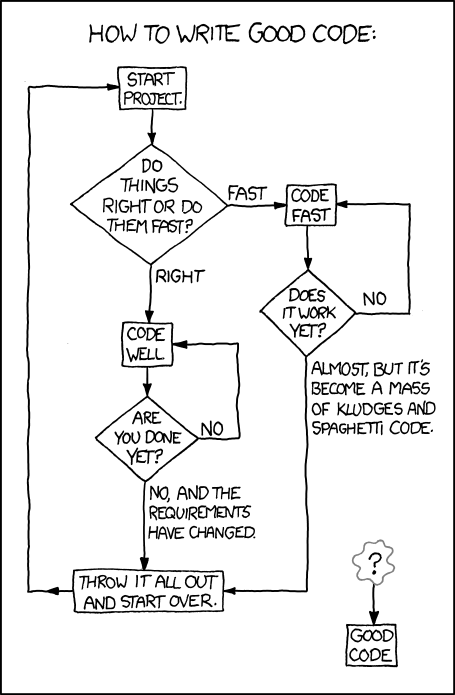
\includegraphics[width=0.6\linewidth]{figs/goodcode.png}
	\caption{Good code? (source: \url{https://xkcd.com/844/})}
	\label{fig:goodcode}
\end{figure}




\section{Writing readable code}

There are a lot of summarized sets of recommended best-practices for writing readable code in general, and for \texttt{R} specifically.
These includes aspects of inline annotation (commenting), object naming conventions (for filenames, function names, and variable names), and syntax and grammar (spacing, indentation, etc.).

In regards to inline annotation, it's rare that code is commented enough.
Believe me, you simply won't remember what certain key lines of code do after even just a few months of working on something else.
Note, however, that comments which simply recapitulate code aren't useful.
Instead of \emph{how}, use annotation that explains \emph{what and why}.

For code grammar and filenames (Figs.~\ref{fig:datafilenames} \& \ref{fig:mapMMDDYYYY}), read Google's Style Guide for R (\textbf{required reading}) before returning to continue reading here.

\url{https://google.github.io/styleguide/Rguide.xml}

\begin{figure}[H]
	\centering
	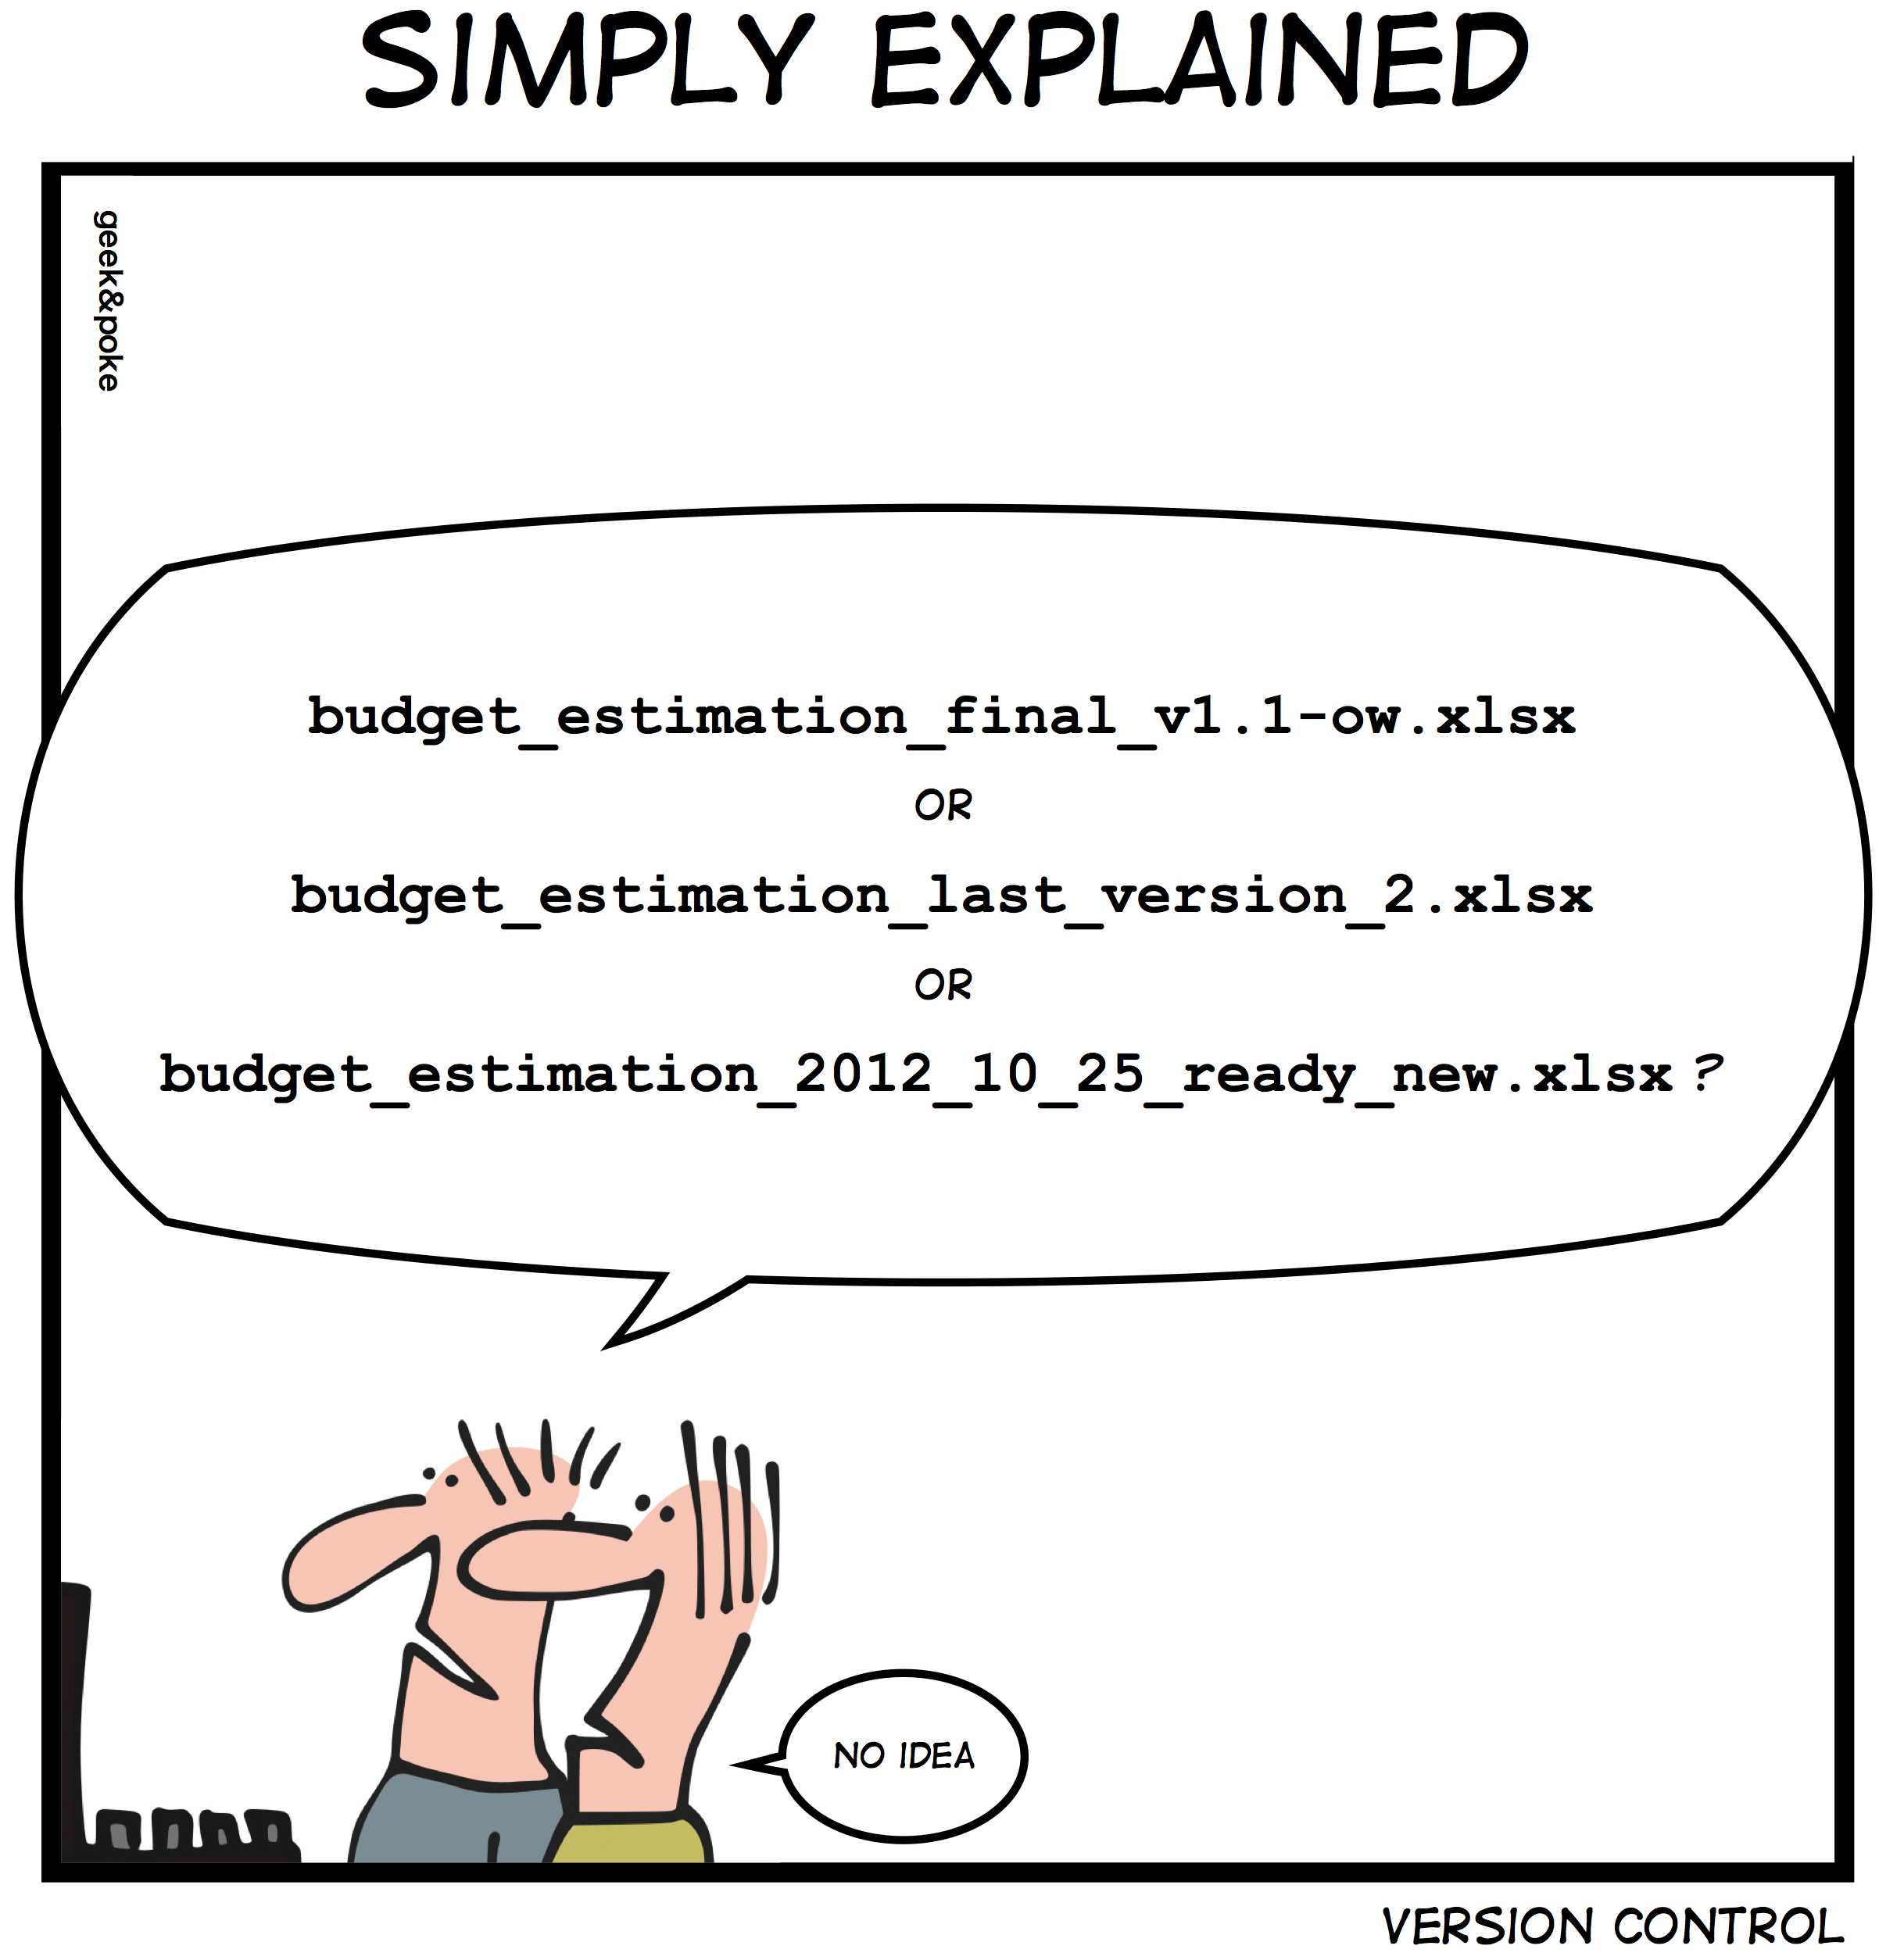
\includegraphics[width=0.6\linewidth]{figs/datafilenames.png}
	\caption{Your data files \emph{will not} look like this; use \texttt{Git}!}
		\label{fig:datafilenames}
\end{figure}

\begin{figure}[H]
	\centering
	
\includegraphics[width=0.6\linewidth]{figs/MapMMDDYYYY.png}
	\caption{A comprehensive map of all countries in the world that use the MMDDYYYY date format; put thought into your filenames. (source: \url{https://twitter.com/donohoe/status/597876118688026624})}
	\label{fig:mapMMDDYYYY}
\end{figure}

Now, even before you become expertly practiced at writing beautifully-readable code (and assuming you're using \texttt{RStudio}), try the following.\footnote{In principal you should really be doing this after initiating a new \texttt{branch} in your \texttt{Git} repository, but we haven't formally learned about branching...yet.}
Highlight some of your code and select \texttt{Code > Reformat Code} from the drop-down menu (or type \texttt{Shift + Cmd/Ctrl + A)}).
\texttt{Reformat code} will try to alter your code to make it adhere to a style guide quite similar to (derived from) Google's style guide.
You'll probably still need to do a little clean-up.
You can also use \texttt{Code > Reindent Lines (Cmd/Ctrl + I)} to clean up nested loops, multi-line functions, and conditional (if-then) sections.\footnote{For even more, try out the styler package (\url{https://github.com/r-lib/styler}).}





\section{When writing code, though shalt also not...}

\begin{itemize}
	\item copy-paste-edit (i.e. reuse and modify) the same code to repeatedly apply it to different subsets of data.  Instead, you will convert your code to function(s) that can be applied to these data subsets.
	\item use \texttt{attach()} and \texttt{detach()} on your data.  Instead, be explicit in naming and accessing data.frame columns.
	\item create large tables by hand. We'll learn \LaTeX\ and export them instead.
\end{itemize}

\begin{figure}
	\centering
	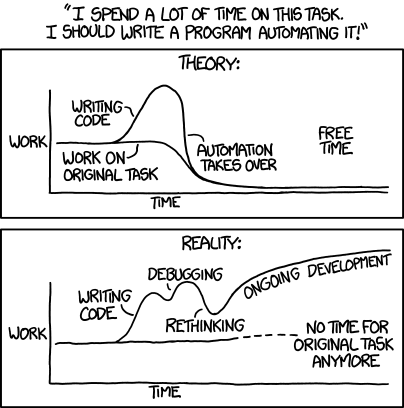
\includegraphics[width=0.7\linewidth]{figs/automation.png}
	\caption{Admittedly, sometimes reality is indeed more like this.  (source: \url{https://xkcd.com/1319/})}
	\label{fig:automation}
\end{figure}




\end{document}
